\documentclass[11pt]{article}
\usepackage[notes]{la}
\lamodule{5}{3}{Diagonalization}
\laxdoc{1.7}
\laxdoc{2.1}
\laxdoc{2.2}
\laxdoc{2.3}
\laxdoc{3.1}
\laxdoc{4.3}
\laxdoc{4.4}
\laxdoc{4.5}
\laxdoc{5.1}
\laxdoc{5.2}

\begin{document}

\section{Diagonalization}

\begin{guide}
A diagonal matrix is the easiest kind of matrix to understand: it multiplies each coordinate by its own number, and its powers are found by raising those numbers to a power. Most matrices are not diagonal, but some of them \emph{behave} like diagonal matrices once we look at them in the right coordinate system. The right coordinate system is a basis of eigenvectors. This section shows exactly when such a basis exists, how to turn it into a factorization $A=PDP^{-1}$, and what goes wrong when it does not exist. The answer rests on one comparison from the last section: for each eigenvalue, the dimension of its eigenspace against its multiplicity as a root.
\end{guide}

\textbf{By the end of this section you should be able to:}
\begin{itemize}
  \item compute $A^k$ from a factorization $A=PDP^{-1}$, and explain why the formula works;
  \item state what it means for a matrix to be diagonalizable, and read the eigenvalues and eigenspace bases of $A$ from a factorization $A=PDP^{-1}$;
  \item diagonalize a matrix when it can be done: find the eigenvalues, a basis for each eigenspace, and assemble $P$ and $D$, in the right order;
  \item decide whether a matrix is diagonalizable, using the number of different eigenvalues, or the dimensions of the eigenspaces compared with the multiplicities;
  \item prove that $\dim E_\lambda$ is never larger than the multiplicity of $\lambda$, and use it to explain why a matrix can fail to be diagonalizable;
  \item build a matrix with prescribed eigenvalues and eigenvectors, and use diagonalization to solve a recurrence;
  \item explain why a real matrix with a non-real eigenvalue is not diagonalizable over the real numbers.
\end{itemize}

% ---------------------------------------------------------------------
\subsection*{Diagonal matrices and their powers}

A \emph{diagonal} matrix has zeros everywhere off the main diagonal. It multiplies the $i$th entry of a vector by its $i$th diagonal entry, and nothing else happens.

\begin{exmp}{Powers of a diagonal matrix}{dpow}
Let $D=\begin{bmatrix}2&0&0\\0&-1&0\\0&0&3\end{bmatrix}$. Multiplying out,
\[
D^2=\begin{bmatrix}2&0&0\\0&-1&0\\0&0&3\end{bmatrix}\begin{bmatrix}2&0&0\\0&-1&0\\0&0&3\end{bmatrix}=\begin{bmatrix}4&0&0\\0&1&0\\0&0&9\end{bmatrix},
\]
and in general $D^k$ is the diagonal matrix with entries $2^k$, $(-1)^k$, $3^k$. For $k=5$ the entries are $32$, $-1$ and $243$. No matrix product is needed: each diagonal entry is raised to the $k$th power by itself.
\end{exmp}

For a matrix that is not diagonal, powers are expensive: each new power is a new matrix product. The idea of this section is that some matrices $A$ can be written as $A=PDP^{-1}$ with $D$ diagonal, and then powers of $A$ cost no more than powers of $D$.

\begin{exmp}{A matrix given by its factorization}{pdp}
Let $P=\begin{bmatrix}2&1\\-3&-1\end{bmatrix}$ and $D=\begin{bmatrix}3&0\\0&4\end{bmatrix}$. Then $\det P=-2+3=1$, so $P$ is invertible with $P^{-1}=\begin{bmatrix}-1&-1\\3&2\end{bmatrix}$, and
\[
PDP^{-1}=\begin{bmatrix}2&1\\-3&-1\end{bmatrix}\begin{bmatrix}3&0\\0&4\end{bmatrix}\begin{bmatrix}-1&-1\\3&2\end{bmatrix}=\begin{bmatrix}6&4\\-9&-4\end{bmatrix}\begin{bmatrix}-1&-1\\3&2\end{bmatrix}=\begin{bmatrix}6&2\\-3&1\end{bmatrix}=A.
\]
Now compare two ways of finding $A^2$. Directly, $A^2=\begin{bmatrix}6&2\\-3&1\end{bmatrix}\begin{bmatrix}6&2\\-3&1\end{bmatrix}=\begin{bmatrix}30&14\\-21&-5\end{bmatrix}$. With the factorization,
\[
A^2=(PDP^{-1})(PDP^{-1})=PD(P^{-1}P)DP^{-1}=PD^2P^{-1}=\begin{bmatrix}2&1\\-3&-1\end{bmatrix}\begin{bmatrix}9&0\\0&16\end{bmatrix}\begin{bmatrix}-1&-1\\3&2\end{bmatrix}=\begin{bmatrix}18&16\\-27&-16\end{bmatrix}\begin{bmatrix}-1&-1\\3&2\end{bmatrix}=\begin{bmatrix}30&14\\-21&-5\end{bmatrix}.
\]
The two answers agree. The middle $P^{-1}P$ cancelled, and that cancellation is the whole trick.
\end{exmp}

\begin{thm}{Powers from a factorization}{powers}
If $A=PDP^{-1}$ with $P$ invertible, then $A^k=PD^kP^{-1}$ for every positive integer $k$. If $D$ is diagonal with diagonal entries $d_1,\dots,d_n$, then $D^k$ is diagonal with diagonal entries $d_1^k,\dots,d_n^k$.
\end{thm}

\begin{proof}
For $k=1$ the formula is the hypothesis. Suppose $A^{k}=PD^{k}P^{-1}$ for some $k\ge1$. Then
\[
A^{k+1}=A^{k}A=(PD^{k}P^{-1})(PDP^{-1})=PD^{k}(P^{-1}P)DP^{-1}=PD^{k+1}P^{-1},
\]
which is the formula for $k+1$. By induction it holds for all $k$. For the second statement, multiplying a diagonal matrix by a diagonal matrix multiplies the diagonal entries and leaves every off-diagonal entry equal to $0$, so by induction the $k$th power of $D$ has the entries $d_i^k$.
\end{proof}

\begin{exmp}{A formula for every power}{closed}
For $A$ of Example~\ref{ex:pdp}, Theorem~\ref{thm:powers} gives
\[
A^k=\begin{bmatrix}2&1\\-3&-1\end{bmatrix}\begin{bmatrix}3^k&0\\0&4^k\end{bmatrix}\begin{bmatrix}-1&-1\\3&2\end{bmatrix}=\begin{bmatrix}2\cdot3^k&4^k\\-3\cdot3^k&-4^k\end{bmatrix}\begin{bmatrix}-1&-1\\3&2\end{bmatrix}=\begin{bmatrix}3\cdot4^k-2\cdot3^k&2\cdot4^k-2\cdot3^k\\3^{k+1}-3\cdot4^k&3^{k+1}-2\cdot4^k\end{bmatrix}.
\]
Check with $k=1$: the entries are $12-6$, $8-6$, $9-12$, $9-8$, which are $6,2,-3,1$, the entries of $A$. \ $\checkmark$ For $k=5$: $3\cdot1024-2\cdot243=2586$ and $2\cdot1024-2\cdot243=1562$, and the second row is $729-3072=-2343$ and $729-2048=-1319$. So $A^5=\begin{bmatrix}2586&1562\\-2343&-1319\end{bmatrix}$, found without computing $A^2,A^3,A^4$.
\end{exmp}

\begin{kc}{Powers from a factorization}{powersk}
Let $A=PDP^{-1}$ with $P=\begin{bmatrix}1&2\\1&3\end{bmatrix}$, $D=\begin{bmatrix}2&0\\0&3\end{bmatrix}$ and $P^{-1}=\begin{bmatrix}3&-2\\-1&1\end{bmatrix}$. (a)~Find $A$. (b)~Find $A^3$ using Theorem~\ref{thm:powers}. (c)~Find a formula for $A^k$.
\end{kc}

\subsection*{What it means to be diagonalizable}

\begin{defn}{Diagonalizable matrix}{diag}
An $n\times n$ matrix $A$ is \emph{diagonalizable} if there are an invertible $n\times n$ matrix $P$ and a diagonal matrix $D$ with $A=PDP^{-1}$. Equivalently $P^{-1}AP=D$, so $A$ is similar to a diagonal matrix (Definition~\ref{5.2-def:similar}).
\end{defn}

When does such a factorization exist? Multiply $A=PDP^{-1}$ on the right by $P$ to get $AP=PD$, and compare columns. Write $P=[\,\bv{p}_1\ \cdots\ \bv{p}_n\,]$ and let $D$ have diagonal entries $d_1,\dots,d_n$. The $j$th column of $AP$ is $A\bv{p}_j$. The $j$th column of $PD$ is $P$ times the $j$th column of $D$, which is $d_j\bv{e}_j$; so it is $d_j\bv{p}_j$. Hence
\[
AP=PD\iff A\bv{p}_j=d_j\bv{p}_j\quad\text{for }j=1,\dots,n.
\]

\begin{think}{Reading the columns}{cols}
(a)~In Example~\ref{ex:pdp}, check that the columns of $P$ are eigenvectors of $A$ by computing $A(2,-3)$ and $A(1,-1)$, and say which eigenvalue goes with which column. (b)~If we swapped the two columns of $P$ and the two diagonal entries of $D$, would $A=PDP^{-1}$ still hold? What if we swapped only the columns of $P$?
\end{think}

\begin{thm}{The Diagonalization Theorem}{diagthm}
An $n\times n$ matrix $A$ is diagonalizable if and only if $A$ has $n$ linearly independent eigenvectors, that is, if and only if $\R^n$ has a basis of eigenvectors of $A$. In that case, $A=PDP^{-1}$ exactly when the columns of $P$ are $n$ linearly independent eigenvectors of $A$ and the diagonal entries of $D$ are the corresponding eigenvalues, in the same order.
\end{thm}

\begin{proof}
Let $P=[\,\bv{p}_1\ \cdots\ \bv{p}_n\,]$ be any $n\times n$ matrix and $D$ the diagonal matrix with diagonal entries $d_1,\dots,d_n$. By the computation above, $AP=PD$ holds exactly when $A\bv{p}_j=d_j\bv{p}_j$ for every $j$.

Suppose $A$ is diagonalizable, $A=PDP^{-1}$. Then $AP=PD$, so each column $\bv{p}_j$ satisfies $A\bv{p}_j=d_j\bv{p}_j$. The matrix $P$ is invertible, so its columns are linearly independent (Theorem~\ref{2.3-thm:imt}) and in particular nonzero. So the $\bv{p}_j$ are $n$ independent eigenvectors, with eigenvalues $d_j$.

Conversely, suppose $\bv{p}_1,\dots,\bv{p}_n$ are independent eigenvectors with $A\bv{p}_j=d_j\bv{p}_j$. Put $P=[\,\bv{p}_1\ \cdots\ \bv{p}_n\,]$ and let $D$ have diagonal entries $d_j$. Then $AP=PD$. The columns of $P$ are independent, so $P$ is invertible (Theorem~\ref{2.3-thm:imt}), and multiplying $AP=PD$ on the right by $P^{-1}$ gives $A=PDP^{-1}$.

The last sentence of the theorem was proved along the way: for an invertible $P$, $A=PDP^{-1}$ forces the columns of $P$ to be eigenvectors with eigenvalues $d_j$, and the converse was just shown. Independent vectors in $\R^n$ with $n$ of them form a basis (Theorem~\ref{4.5-thm:basis}), which gives the statement about a basis.
\end{proof}

\begin{exmp}{Diagonalizing a $2\times2$ matrix}{twoby}
Let $A=\begin{bmatrix}0&3\\2&1\end{bmatrix}$. Here $\operatorname{tr}A=1$ and $\det A=-6$, so $p_A(\lambda)=\lambda^2-\lambda-6=(\lambda-3)(\lambda+2)$ (Theorem~\ref{5.2-thm:shape}). The eigenvalues are $3$ and $-2$. For $\lambda=3$,
\begin{align*}
\begin{amat}{cc|c}-3 & 3 & 0\\2 & -2 & 0\end{amat}
&\rops{-\tfrac{1}{3}R_1}
\begin{amat}{cc|c}1 & -1 & 0\\2 & -2 & 0\end{amat}
\rops{R_2-2R_1}
\begin{amat}{cc|c}1 & -1 & 0\\0 & 0 & 0\end{amat}
\end{align*}
so $x_1=x_2$ and $(1,1)$ is an eigenvector. For $\lambda=-2$,
\begin{align*}
\begin{amat}{cc|c}2 & 3 & 0\\2 & 3 & 0\end{amat}
&\rops{\tfrac{1}{2}R_1}
\begin{amat}{cc|c}1 & \tfrac{3}{2} & 0\\2 & 3 & 0\end{amat}
\rops{R_2-2R_1}
\begin{amat}{cc|c}1 & \tfrac{3}{2} & 0\\0 & 0 & 0\end{amat}
\end{align*}
so $x_1=-\tfrac32x_2$, and taking $x_2=-2$ gives the eigenvector $(3,-2)$. The two eigenvectors belong to different eigenvalues, so they are independent (Theorem~\ref{5.1-thm:indep}). By Theorem~\ref{thm:diagthm}, $A$ is diagonalizable, with
\[
P=\begin{bmatrix}1&3\\1&-2\end{bmatrix},\qquad D=\begin{bmatrix}3&0\\0&-2\end{bmatrix}.
\]
Check $AP=PD$, which avoids finding $P^{-1}$: $AP=\begin{bmatrix}0&3\\2&1\end{bmatrix}\begin{bmatrix}1&3\\1&-2\end{bmatrix}=\begin{bmatrix}3&-6\\3&4\end{bmatrix}$ and $PD=\begin{bmatrix}1&3\\1&-2\end{bmatrix}\begin{bmatrix}3&0\\0&-2\end{bmatrix}=\begin{bmatrix}3&-6\\3&4\end{bmatrix}$. \ $\checkmark$ The order matters: the first column of $P$ goes with the first diagonal entry of $D$, and so on.
\end{exmp}

\begin{proc}{Diagonalizing an $n\times n$ matrix}{diag}
\begin{enumerate}[itemsep=1pt]
  \item Find the eigenvalues of $A$: the roots of $p_A(\lambda)=\det(A-\lambda I)$ (Procedure~\ref{5.2-proc:find}).
  \item For each eigenvalue $\lambda_0$, find a basis of $E_{\lambda_0}=\Nul(A-\lambda_0I)$ by row reducing $[\,A-\lambda_0I\ \ \bv{0}\,]$ (Procedure~\ref{5.1-proc:eigspace}).
  \item Collect all the basis vectors found. If there are fewer than $n$ of them, $A$ is \emph{not} diagonalizable (Theorem~\ref{thm:criterion}). If there are $n$, they are independent (Theorem~\ref{thm:union}).
  \item Put them as the columns of $P$ in any order, and put the corresponding eigenvalues on the diagonal of $D$ in the same order, each repeated as many times as it has basis vectors.
  \item Check $AP=PD$. This confirms the arithmetic without computing $P^{-1}$.
\end{enumerate}
\end{proc}

\begin{exmp}{A $3\times3$ matrix with three different eigenvalues}{three}
Let $A=\begin{bmatrix}2&3&-1\\1&4&5\\0&0&-2\end{bmatrix}$. The third row has two zeros, so expanding $\det(A-\lambda I)$ along it,
\[
\det(A-\lambda I)=(-2-\lambda)\begin{vmatrix}2-\lambda&3\\1&4-\lambda\end{vmatrix}=(-2-\lambda)(\lambda^2-6\lambda+5)=-(\lambda+2)(\lambda-1)(\lambda-5).
\]
The eigenvalues are $-2$, $1$ and $5$: three different eigenvalues for a $3\times3$ matrix, so $A$ is diagonalizable (this is Theorem~\ref{thm:distinct} below; here we just go on). Eigenvectors:
\begin{align*}
\lambda=5:&\quad\begin{amat}{ccc|c}-3 & 3 & -1 & 0\\1 & -1 & 5 & 0\\0 & 0 & -7 & 0\end{amat}\ \text{has reduced form}\ \begin{amat}{ccc|c}1 & -1 & 0 & 0\\0 & 0 & 1 & 0\\0 & 0 & 0 & 0\end{amat},\quad E_5=\Span\{(1,1,0)\},\\
\lambda=1:&\quad\begin{amat}{ccc|c}1 & 3 & -1 & 0\\1 & 3 & 5 & 0\\0 & 0 & -3 & 0\end{amat}\ \text{has reduced form}\ \begin{amat}{ccc|c}1 & 3 & 0 & 0\\0 & 0 & 1 & 0\\0 & 0 & 0 & 0\end{amat},\quad E_1=\Span\{(-3,1,0)\},\\
\lambda=-2:&\quad\begin{amat}{ccc|c}4 & 3 & -1 & 0\\1 & 6 & 5 & 0\\0 & 0 & 0 & 0\end{amat}\ \text{has reduced form}\ \begin{amat}{ccc|c}1 & 0 & -1 & 0\\0 & 1 & 1 & 0\\0 & 0 & 0 & 0\end{amat},\quad E_{-2}=\Span\{(1,-1,1)\}.
\end{align*}
(For $\lambda=-2$ the free variable is $x_3$, with $x_1=x_3$ and $x_2=-x_3$.) Take $\bv{p}_1=(1,1,0)$, $\bv{p}_2=(-3,1,0)$, $\bv{p}_3=(1,-1,1)$ with eigenvalues $5,1,-2$:
\[
P=\begin{bmatrix}1&-3&1\\1&1&-1\\0&0&1\end{bmatrix},\qquad D=\begin{bmatrix}5&0&0\\0&1&0\\0&0&-2\end{bmatrix}.
\]
Check $AP=PD$: the columns of $AP$ are $A\bv{p}_1=(5,5,0)$, $A\bv{p}_2=(-3,1,0)$ and $A\bv{p}_3=(-2,2,-2)$, which are $5\bv{p}_1$, $1\cdot\bv{p}_2$ and $-2\bv{p}_3$. \ $\checkmark$
\end{exmp}

\begin{kc}{Diagonalize}{dok}
Let $A=\begin{bmatrix}1&2\\3&0\end{bmatrix}$. (a)~Find the eigenvalues of $A$ and an eigenvector for each. (b)~Write down $P$ and $D$ with $A=PDP^{-1}$. (c)~Check your answer by computing $AP$ and $PD$. (d)~Write another valid pair $P$, $D$.
\end{kc}

% ---------------------------------------------------------------------
\subsection*{When there are enough eigenvalues, and when there are not}

The easy case was met already in Section~5.1: eigenvectors for different eigenvalues are independent, so $n$ different eigenvalues give $n$ independent eigenvectors.

\begin{thm}{Different eigenvalues suffice}{distinct}
If an $n\times n$ matrix has $n$ different eigenvalues, then it is diagonalizable.
\end{thm}

\begin{proof}
Choose one eigenvector for each of the $n$ eigenvalues. By Theorem~\ref{5.1-thm:indep}, they are linearly independent, so $A$ has $n$ independent eigenvectors. By the Diagonalization Theorem (Theorem~\ref{thm:diagthm}), $A$ is diagonalizable.
\end{proof}

\begin{exmp}{A triangular matrix with different diagonal entries}{tridist}
Let $T=\begin{bmatrix}2&7&1\\0&-1&4\\0&0&5\end{bmatrix}$. By Theorem~\ref{5.1-thm:tri} the eigenvalues of a triangular matrix are its diagonal entries, here $2$, $-1$ and $5$, which are different. By Theorem~\ref{thm:distinct}, $T$ is diagonalizable, and we know this before finding a single eigenvector. The eigenvectors (and so $P$) are found by row reducing, but we do not need them to answer the \emph{question}. In contrast, the matrix $\begin{bmatrix}2&7&1\\0&-1&4\\0&0&2\end{bmatrix}$ has a repeated diagonal entry, and Theorem~\ref{thm:distinct} says nothing about it.
\end{exmp}

\begin{think}{Only sufficient}{suff}
(a)~The identity matrix $I_3$ has only one eigenvalue. Is it diagonalizable? What is $P$? (b)~What does this say about the converse of Theorem~\ref{thm:distinct}? (c)~Why is the argument ``$n$ different eigenvalues, so $n$ independent eigenvectors'' not available when an eigenvalue is repeated?
\end{think}

When an eigenvalue is repeated, everything depends on its eigenspace. We have met both outcomes.

\begin{exmp}{A repeated eigenvalue that is harmless}{repyes}
Let $A=\begin{bmatrix}3&0&0\\2&1&-2\\2&-2&1\end{bmatrix}$. Expanding along the first row, $\det(A-\lambda I)=(3-\lambda)\bigl[(1-\lambda)^2-4\bigr]=(3-\lambda)(-1-\lambda)(3-\lambda)$, so $p_A(\lambda)=-(\lambda-3)^2(\lambda+1)$: the eigenvalue $3$ has multiplicity $2$. For $\lambda=3$:
\begin{align*}
\begin{amat}{ccc|c}0 & 0 & 0 & 0\\2 & -2 & -2 & 0\\2 & -2 & -2 & 0\end{amat}
&\rops{R_1\leftrightarrow R_2}
\begin{amat}{ccc|c}2 & -2 & -2 & 0\\0 & 0 & 0 & 0\\2 & -2 & -2 & 0\end{amat}
\rops{\tfrac{1}{2}R_1}
\begin{amat}{ccc|c}1 & -1 & -1 & 0\\0 & 0 & 0 & 0\\2 & -2 & -2 & 0\end{amat}
\\[4pt]
&\rops{R_3-2R_1}
\begin{amat}{ccc|c}1 & -1 & -1 & 0\\0 & 0 & 0 & 0\\0 & 0 & 0 & 0\end{amat}
\end{align*}
There are two free variables, $x_2$ and $x_3$, and $x_1=x_2+x_3$. So $E_3=\Span\{(1,1,0),(1,0,1)\}$ has dimension $2$. For $\lambda=-1$, the matrix $A+I=\begin{bmatrix}4&0&0\\2&2&-2\\2&-2&2\end{bmatrix}$ forces $x_1=0$ and $x_2=x_3$, so $E_{-1}=\Span\{(0,1,1)\}$. Altogether we have $2+1=3$ eigenvectors. They are independent (Theorem~\ref{thm:union} below), so $A$ is diagonalizable, with
\[
P=\begin{bmatrix}1&1&0\\1&0&1\\0&1&1\end{bmatrix},\qquad D=\begin{bmatrix}3&0&0\\0&3&0\\0&0&-1\end{bmatrix}.
\]
Check: $A(1,1,0)=(3,3,0)$, $A(1,0,1)=(3,0,3)$ and $A(0,1,1)=(0,-1,-1)$. \ $\checkmark$
\end{exmp}

\begin{exmp}{A repeated eigenvalue that is fatal}{repno}
Let $B=\begin{bmatrix}3&0&0\\2&1&2\\-2&0&1\end{bmatrix}$. Expanding along the first row, $p_B(\lambda)=(3-\lambda)(1-\lambda)^2$, so the eigenvalue $1$ has multiplicity $2$. For $\lambda=1$,
\begin{align*}
B-I=\begin{bmatrix}2&0&0\\2&0&2\\-2&0&0\end{bmatrix}
&\rightarrow\begin{amat}{ccc|c}1 & 0 & 0 & 0\\0 & 0 & 1 & 0\\0 & 0 & 0 & 0\end{amat}
\end{align*}
as one checks by row reducing. Only $x_2$ is free, with $x_1=x_3=0$, so $E_1=\Span\{(0,1,0)\}$ has dimension $1$. For $\lambda=3$ the eigenspace is $E_3=\Span\{(-1,0,1)\}$, again a line. In total there are only $1+1=2$ independent eigenvectors, and a $3\times3$ matrix needs $3$. By the Diagonalization Theorem, $B$ is \emph{not} diagonalizable. There is no room for a third independent eigenvector: every eigenvector of $B$ lies in $E_1$ or $E_3$, and those are two lines.
\end{exmp}

\begin{exmp}{A $2\times2$ matrix that is not diagonalizable}{shear}
Let $S=\begin{bmatrix}1&-1\\1&3\end{bmatrix}$. Then $\operatorname{tr}S=4$ and $\det S=4$, so $p_S(\lambda)=\lambda^2-4\lambda+4=(\lambda-2)^2$: the only eigenvalue is $2$, with multiplicity $2$. Now $S-2I=\begin{bmatrix}-1&-1\\1&1\end{bmatrix}$ has rank $1$, so $E_2=\Span\{(1,-1)\}$ is a line. Every eigenvector of $S$ is a multiple of $(1,-1)$, so $\R^2$ has no basis of eigenvectors, and $S$ is not diagonalizable. (If $S$ were diagonalizable with the only eigenvalue $2$, we would have $S=P(2I)P^{-1}=2I$; but $S\neq2I$. This is the same argument as Example~\ref{5.2-ex:notsim}.)
\end{exmp}

\begin{kc}{Enough eigenvectors?}{enough}
For each matrix, say how many independent eigenvectors there are and whether the matrix is diagonalizable. (a)~$\begin{bmatrix}5&1\\0&5\end{bmatrix}$. (b)~$\begin{bmatrix}5&0\\0&5\end{bmatrix}$. (c)~$\begin{bmatrix}4&0&0\\0&7&1\\0&0&7\end{bmatrix}$. (d)~$\begin{bmatrix}1&2&3\\0&4&5\\0&0&6\end{bmatrix}$.
\end{kc}

% ---------------------------------------------------------------------
\subsection*{Eigenspaces against multiplicities}

Examples~\ref{ex:repyes} and~\ref{ex:repno} have the same kind of characteristic polynomial, a double root and a simple root, and different outcomes. The difference is the dimension of the eigenspace of the double root. We now name the two numbers that are being compared.

\begin{defn}{Algebraic and geometric multiplicity}{twomult}
Let $\lambda_0$ be an eigenvalue of the $n\times n$ matrix $A$. Its \emph{algebraic multiplicity} is its multiplicity as a root of $p_A$ (Definition~\ref{5.2-def:mult}). Its \emph{geometric multiplicity} is $\dim E_{\lambda_0}=\dim\Nul(A-\lambda_0I)$, the number of free variables in $(A-\lambda_0I)\bv{x}=\bv{0}$.
\end{defn}

In Example~\ref{ex:repyes} the eigenvalue $3$ has algebraic multiplicity $2$ and geometric multiplicity $2$; in Example~\ref{ex:repno} the eigenvalue $1$ has algebraic multiplicity $2$ and geometric multiplicity $1$. Two facts hold for every matrix. First, eigenspaces for different eigenvalues do not interfere with each other.

\begin{thm}{Bases of different eigenspaces fit together}{union}
Let $\lambda_1,\dots,\lambda_r$ be different eigenvalues of $A$, and for each $i$ let $S_i$ be a linearly independent set in $E_{\lambda_i}$. Then the set $S_1\cup\cdots\cup S_r$ is linearly independent. In particular, if each $S_i$ is a basis for $E_{\lambda_i}$, the union is independent.
\end{thm}

\begin{proof}
Write $S_i=\{\bv{v}_{i1},\dots,\bv{v}_{im_i}\}$ and suppose a combination of all the vectors is $\bv{0}$:
\[
\bv{w}_1+\bv{w}_2+\cdots+\bv{w}_r=\bv{0},\qquad\text{where }\bv{w}_i=c_{i1}\bv{v}_{i1}+\cdots+c_{im_i}\bv{v}_{im_i}\ \text{ lies in }E_{\lambda_i}.
\]
Each $\bv{w}_i$ is in the subspace $E_{\lambda_i}$ (Theorem~\ref{5.1-thm:eigsub}), so each $\bv{w}_i$ is either $\bv{0}$ or an eigenvector for $\lambda_i$. Suppose some $\bv{w}_i$ is not $\bv{0}$, and discard the zero ones. What remains is a nonempty list of eigenvectors for \emph{different} eigenvalues whose sum is $\bv{0}$, that is, a linear dependence relation with all weights equal to $1$. But eigenvectors for different eigenvalues are linearly independent (Theorem~\ref{5.1-thm:indep}), which allows no such relation. Hence every $\bv{w}_i=\bv{0}$. For a fixed $i$, $\bv{w}_i=\bv{0}$ is a combination of the independent set $S_i$, so all $c_{ij}=0$. Thus only the trivial combination of the whole union gives $\bv{0}$.
\end{proof}

Second, the geometric multiplicity can never exceed the algebraic one. This is the fact that Pause and think~\ref{5.2-think:twonumbers} suggested; we now prove it in general.

\begin{thm}{Eigenspace dimension is at most the multiplicity}{dimmult}
Let $\lambda_0$ be an eigenvalue of an $n\times n$ matrix $A$. Then $\dim E_{\lambda_0}$ is at most the algebraic multiplicity of $\lambda_0$.
\end{thm}

\begin{proof}
Let $k=\dim E_{\lambda_0}$ and let $\bv{v}_1,\dots,\bv{v}_k$ be a basis of $E_{\lambda_0}$. Extend it to a basis $\bv{v}_1,\dots,\bv{v}_n$ of $\R^n$ (Procedure~\ref{4.5-proc:extend}) and let $P=[\,\bv{v}_1\ \cdots\ \bv{v}_n\,]$, which is invertible. Put $B=P^{-1}AP$.

\emph{The shape of $B$.} For $j\le k$, the $j$th column of $AP$ is $A\bv{v}_j=\lambda_0\bv{v}_j=\lambda_0P\bv{e}_j$, so the $j$th column of $B=P^{-1}(AP)$ is $P^{-1}\lambda_0P\bv{e}_j=\lambda_0\bv{e}_j$. So the first $k$ columns of $B$ have $\lambda_0$ on the diagonal and zeros elsewhere:
\[
B=\begin{bmatrix}\lambda_0I_k&X\\O&C\end{bmatrix},
\]
where $X$ is $k\times(n-k)$, $O$ is a zero block and $C$ is $(n-k)\times(n-k)$.

\emph{The characteristic polynomial.} The matrix $B-\lambda I$ has the same block shape, with $(\lambda_0-\lambda)I_k$ in the upper left corner and $C-\lambda I$ in the lower right. The first column of $B-\lambda I$ has only one nonzero entry, $\lambda_0-\lambda$ at the top, so expanding along the first column (Theorem~\ref{3.1-thm:expansion}) gives $(\lambda_0-\lambda)$ times the determinant of the matrix with the first row and column deleted, which has the same block shape with $k-1$ in place of $k$. Repeating this $k$ times,
\[
p_B(\lambda)=(\lambda_0-\lambda)^k\det(C-\lambda I)=(\lambda_0-\lambda)^k\,p_C(\lambda).
\]
\emph{Conclusion.} $A$ and $B$ are similar, so $p_A=p_B$ (Theorem~\ref{5.2-thm:similar}). Hence $(\lambda-\lambda_0)^k$ divides $p_A(\lambda)$, so the multiplicity of $\lambda_0$ as a root of $p_A$ is at least $k$.
\end{proof}

\begin{exmp}{The block shape in a numerical case}{blockform}
Take $A$ of Example~\ref{ex:repyes}, where $E_3$ has the basis $\bv{v}_1=(1,1,0)$, $\bv{v}_2=(1,0,1)$ and $k=2$. Extend by $\bv{v}_3=(0,0,1)$: the matrix $P=\begin{bmatrix}1&1&0\\1&0&0\\0&1&1\end{bmatrix}$ has $\det P=-1$, so $\bv{v}_1,\bv{v}_2,\bv{v}_3$ is a basis of $\R^3$. Then
\[
P^{-1}AP=\begin{bmatrix}3&0&-2\\0&3&2\\0&0&-1\end{bmatrix}.
\]
The first two columns are $3\bv{e}_1$ and $3\bv{e}_2$, as in the proof, and the lower right block is $C=[-1]$, whose characteristic polynomial is $-1-\lambda$. So $p_A(\lambda)=(3-\lambda)^2(-1-\lambda)$, which is what we found by expanding $\det(A-\lambda I)$ directly. The new vector $\bv{v}_3$ is \emph{not} an eigenvector; the last column of the new matrix records that $A\bv{v}_3=-2\bv{v}_1+2\bv{v}_2-\bv{v}_3$.
\end{exmp}

\begin{think}{Why the bound holds}{whybound}
(a)~In Example~\ref{ex:blockform}, which entries of $P^{-1}AP$ record that $\bv{v}_1$ and $\bv{v}_2$ are eigenvectors? (b)~If $k=n$ in the proof, what is $B$, and what does the theorem say? (c)~Does the theorem tell you that $\dim E_{\lambda_0}$ equals the multiplicity? Give an example from this section.
\end{think}

Together these two theorems decide diagonalizability for every matrix.

\begin{thm}{When is a matrix diagonalizable?}{criterion}
Let $A$ be an $n\times n$ matrix with real entries. The following are equivalent.
\begin{enumerate}[label=(\alph*),itemsep=1pt]
  \item $A$ is diagonalizable.
  \item The dimensions of the eigenspaces of $A$ (over the different real eigenvalues) add up to $n$.
  \item The multiplicities of the real eigenvalues add up to $n$ (so $p_A$ splits into real linear factors), and for every eigenvalue the geometric multiplicity equals the algebraic multiplicity.
\end{enumerate}
\end{thm}

\begin{proof}
Let $\lambda_1,\dots,\lambda_r$ be the different real eigenvalues, with $d_i=\dim E_{\lambda_i}$ and algebraic multiplicities $m_i$.

(a)$\Rightarrow$(b). By Theorem~\ref{thm:diagthm}, $\R^n$ has a basis of eigenvectors. Sort the basis vectors by eigenvalue; those for $\lambda_i$ lie in $E_{\lambda_i}$ and are independent, so there are at most $d_i$ of them. Hence $n\le d_1+\cdots+d_r$. On the other hand, bases of the eigenspaces fit together into an independent set (Theorem~\ref{thm:union}), and an independent set in $\R^n$ has at most $n$ vectors (Theorem~\ref{1.7-thm:count}), so $d_1+\cdots+d_r\le n$. Thus the sum is $n$.

(b)$\Rightarrow$(a). The union of bases of the eigenspaces is independent (Theorem~\ref{thm:union}) and has $d_1+\cdots+d_r=n$ vectors, so it is a set of $n$ independent eigenvectors, and $A$ is diagonalizable by Theorem~\ref{thm:diagthm}.

(b)$\Rightarrow$(c). By Theorem~\ref{thm:dimmult}, $d_i\le m_i$, and $m_1+\cdots+m_r\le n$ because the degree of $p_A$ is $n$ (Theorem~\ref{5.2-thm:shape}). So $n=\sum d_i\le\sum m_i\le n$. Equality holds throughout, which gives $\sum m_i=n$ and, since each $d_i\le m_i$, $d_i=m_i$ for every $i$.

(c)$\Rightarrow$(b). If $d_i=m_i$ for all $i$, then $\sum d_i=\sum m_i=n$.
\end{proof}

Real eigenvalues need not be all the roots. A real matrix may have non-real roots of $p_A$ (Section~5.2); then (c) fails, and $A$ is not diagonalizable \emph{over the real numbers}. This is the case of a rotation, Example~\ref{ex:rot} below.

\begin{proc}{Deciding whether a matrix is diagonalizable}{decide}
\begin{enumerate}[itemsep=1pt]
  \item Find $p_A$ and factor it. If it has a non-real root, $A$ is not diagonalizable over $\R$. If it has $n$ different real roots, $A$ is diagonalizable (Theorem~\ref{thm:distinct}).
  \item Otherwise some root has multiplicity $m\ge2$. For each such root $\lambda_0$, find $\dim E_{\lambda_0}=n-\rank(A-\lambda_0I)$.
  \item $A$ is diagonalizable if and only if $\dim E_{\lambda_0}=m$ for every repeated root (Theorem~\ref{thm:criterion}). One eigenvalue with $\dim E_{\lambda_0}<m$ is enough to say no.
\end{enumerate}
\end{proc}

(For a simple root, $1\le\dim E_\lambda\le1$, so nothing needs checking.)

\begin{exmp}{A parameter decides}{param}
Let $A_h=\begin{bmatrix}2&1&0\\0&h&0\\0&0&2\end{bmatrix}$. For which $h$ is $A_h$ diagonalizable? The matrix is triangular, so its eigenvalues are $2$, $h$ and $2$.

\emph{If $h\neq2$:} the eigenvalue $2$ has multiplicity $2$, and $h$ is a simple eigenvalue. Now $A_h-2I=\begin{bmatrix}0&1&0\\0&h-2&0\\0&0&0\end{bmatrix}$ has rank $1$ (its two nonzero rows are proportional, because $(0,h-2,0)=(h-2)(0,1,0)$), so $\dim E_2=3-1=2$, equal to the multiplicity. By Theorem~\ref{thm:criterion}, $A_h$ is diagonalizable.

\emph{If $h=2$:} the eigenvalue $2$ has multiplicity $3$, and $A_2-2I=\begin{bmatrix}0&1&0\\0&0&0\\0&0&0\end{bmatrix}$ has rank $1$, so $\dim E_2=2<3$. By Theorem~\ref{thm:criterion}, $A_2$ is \emph{not} diagonalizable.

So $A_h$ is diagonalizable exactly when $h\neq2$. The multiplicity of $2$ jumped from $2$ to $3$ at $h=2$, while the eigenspace stayed two-dimensional.
\end{exmp}

\begin{kc}{Decide}{decidek}
In each case decide whether $A$ is diagonalizable over $\R$, and say why. (a)~$A$ is $4\times4$, $p_A(\lambda)=(\lambda-2)^3(\lambda+1)$, $\dim E_2=2$ and $\dim E_{-1}=1$. (b)~The same $p_A$ with $\dim E_2=3$. (c)~$A$ is $4\times4$ with $p_A(\lambda)=(\lambda^2+1)(\lambda-3)(\lambda+1)$. (d)~$A$ is $5\times5$ with the eigenvalues $1,2,3,4,5$.
\end{kc}

\subsection*{Eigenvectors as a coordinate system}

The factorization $A=PDP^{-1}$ has a meaning that goes beyond arithmetic. Let $\mathcal{B}=\{\bv{p}_1,\dots,\bv{p}_n\}$ be the basis of eigenvectors, so that $P=P_{\mathcal{B}}$ is the matrix of Section~4.4 with $\bv{x}=P[\bv{x}]_{\mathcal{B}}$ and $[\bv{x}]_{\mathcal{B}}=P^{-1}\bv{x}$ (Theorem~\ref{4.4-thm:PB}). Then $A\bv{x}=PDP^{-1}\bv{x}$ reads: \emph{translate $\bv{x}$ into $\mathcal{B}$-coordinates, multiply each coordinate by its eigenvalue, and translate back.}

\begin{exmp}{Computing in eigenvector coordinates}{coord}
Take $A=\begin{bmatrix}6&2\\-3&1\end{bmatrix}$ of Example~\ref{ex:pdp}, with eigenvectors $\bv{p}_1=(2,-3)$ for $3$ and $\bv{p}_2=(1,-1)$ for $4$, and $\bv{x}=(5,-6)$. The coordinates of $\bv{x}$ are $P^{-1}\bv{x}=\begin{bmatrix}-1&-1\\3&2\end{bmatrix}\begin{bmatrix}5\\-6\end{bmatrix}=\begin{bmatrix}1\\3\end{bmatrix}$, so $\bv{x}=1\cdot\bv{p}_1+3\bv{p}_2$. In these coordinates $A$ multiplies the first by $3$ and the second by $4$: $A\bv{x}=3\bv{p}_1+12\bv{p}_2=(6,-9)+(12,-12)=(18,-21)$. Directly, $A\bv{x}=(30-12,\ -15-6)=(18,-21)$. \ $\checkmark$ After $k$ steps the coordinates are $(3^k,\ 3\cdot4^k)$.
\end{exmp}

\begin{center}
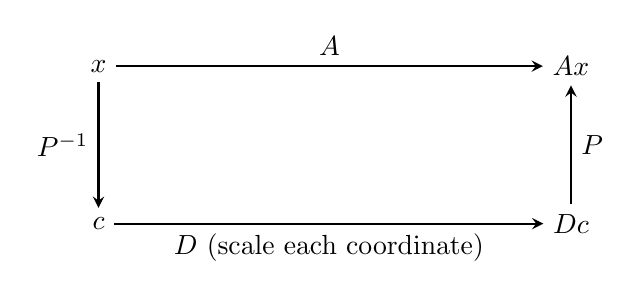
\begin{tikzpicture}[>=stealth,node distance=2.6cm]
  \node (x) at (0,2) {$x$};
  \node (Ax) at (6,2) {$Ax$};
  \node (c) at (0,0) {$c$};
  \node (Dc) at (6,0) {$Dc$};
  \draw[->,thick] (x)--(Ax) node[midway,above] {$A$};
  \draw[->,thick] (c)--(Dc) node[midway,below] {$D$ (scale each coordinate)};
  \draw[->,thick] (x)--(c) node[midway,left] {$P^{-1}$};
  \draw[->,thick] (Dc)--(Ax) node[midway,right] {$P$};
\end{tikzpicture}
\end{center}

\noindent\textbf{Figure 1.} Two routes from $\bv{x}$ to $A\bv{x}$: apply $A$ directly, or go down to the coordinates $\bv{c}=P^{-1}\bv{x}$, scale them by $D$, and come back up by $P$. The two routes give the same vector because $A=PDP^{-1}$.

\begin{think}{Straight lines of eigenvectors}{lines}
(a)~In Example~\ref{ex:coord}, what does $A$ do to the line through $\bv{p}_1$? Through $\bv{p}_2$? (b)~If all eigenvalues are larger than $1$ in size, what happens to every vector under repeated application of $A$? (c)~Why does Figure~1 need $P$ to be invertible?
\end{think}

\begin{exmp}{A recurrence solved by diagonalization}{recur}
The sequence $a_0=2$, $a_1=1$, $a_{k+2}=a_{k+1}+6a_k$ begins $2,1,13,19,97,\dots$. Put $\bv{x}_k=(a_{k+1},a_k)$. Then $\bv{x}_{k+1}=(a_{k+2},a_{k+1})=(a_{k+1}+6a_k,\ a_{k+1})=C\bv{x}_k$ with $C=\begin{bmatrix}1&6\\1&0\end{bmatrix}$, so $\bv{x}_k=C^k\bv{x}_0$ with $\bv{x}_0=(1,2)$. Now $\operatorname{tr}C=1$ and $\det C=-6$, so $p_C(\lambda)=\lambda^2-\lambda-6=(\lambda-3)(\lambda+2)$. Eigenvectors: $(3,1)$ for $3$ (since $C(3,1)=(3+6,3)=(9,3)$) and $(-2,1)$ for $-2$ (since $C(-2,1)=(-2+6,-2)=(4,-2)$). Write $\bv{x}_0=c_1(3,1)+c_2(-2,1)$: $3c_1-2c_2=1$ and $c_1+c_2=2$ give $c_1=c_2=1$. Therefore
\[
\bv{x}_k=3^k\begin{bmatrix}3\\1\end{bmatrix}+(-2)^k\begin{bmatrix}-2\\1\end{bmatrix},\qquad\text{so}\qquad a_k=3^k+(-2)^k.
\]
Check: $a_2=9+4=13$ and $a_3=27-8=19$. \ $\checkmark$ For large $k$, $a_{k+1}/a_k$ is close to $3$, the larger eigenvalue.
\end{exmp}

\begin{exmp}{Building a matrix from eigenvectors}{build}
Find a $2\times2$ matrix $A$ with $A(1,1)=2(1,1)$ and $A(1,2)=-1\cdot(1,2)$. The vectors $(1,1)$ and $(1,2)$ are independent, so $P=\begin{bmatrix}1&1\\1&2\end{bmatrix}$ ($\det P=1$, $P^{-1}=\begin{bmatrix}2&-1\\-1&1\end{bmatrix}$) and $D=\begin{bmatrix}2&0\\0&-1\end{bmatrix}$ satisfy the conditions of Theorem~\ref{thm:diagthm}, and
\[
A=PDP^{-1}=\begin{bmatrix}1&1\\1&2\end{bmatrix}\begin{bmatrix}2&0\\0&-1\end{bmatrix}\begin{bmatrix}2&-1\\-1&1\end{bmatrix}=\begin{bmatrix}2&-1\\2&-2\end{bmatrix}\begin{bmatrix}2&-1\\-1&1\end{bmatrix}=\begin{bmatrix}5&-3\\6&-4\end{bmatrix}.
\]
Check: $A(1,1)=(2,2)$ and $A(1,2)=(5-6,\ 6-8)=(-1,-2)$. \ $\checkmark$ This is the only such matrix, because $A$ is determined on a basis, and a linear map is determined by what it does to a basis.
\end{exmp}

\begin{kc}{Build a matrix}{buildk}
Find a $2\times2$ matrix $A$ with $A(1,0)=3(1,0)$ and $A(1,1)=5(1,1)$. Then compute $A^k$.
\end{kc}

\subsection*{Matrices with no real eigenvalues}

\begin{exmp}{A rotation is not diagonalizable over $\R$}{rot}
The rotation $R=\begin{bmatrix}0&-1\\1&0\end{bmatrix}$ through $90^\circ$ has $p_R(\lambda)=\lambda^2+1$, whose roots $\pm i$ are not real (Example~\ref{5.1-ex:geom}(d)). By Theorem~\ref{thm:criterion} it is not diagonalizable over $\R$; geometrically, no line through the origin is mapped to itself. Over the complex numbers, however, the eigenvalues $i$ and $-i$ are different, with eigenvectors $(1,-i)$ for $i$ (check: $R(1,-i)=(i,1)=i\,(1,-i)$) and $(1,i)$ for $-i$. The Diagonalization Theorem is true with complex numbers in place of real ones, so $R=PDP^{-1}$ with $P=\begin{bmatrix}1&1\\-i&i\end{bmatrix}$ and $D=\begin{bmatrix}i&0\\0&-i\end{bmatrix}$. Then $R^4=PD^4P^{-1}=PIP^{-1}=I$, as it should be for four quarter turns.
\end{exmp}

\begin{think}{Real or complex}{cplxthink}
(a)~Which hypothesis of the Diagonalization Theorem fails for $R$ over $\R$, and which holds over $\C$? (b)~Is every real $2\times2$ matrix with two different complex eigenvalues diagonalizable over $\C$? Use Theorem~\ref{thm:distinct}. (c)~A real $3\times3$ matrix always has a real eigenvalue (Section~5.2). Can it fail to be diagonalizable over $\R$ for reasons of non-real roots?
\end{think}

\begin{think}{Long-term behaviour}{limit}
Let $A=PDP^{-1}$ with $D=\operatorname{diag}(1,\tfrac12,\tfrac13)$. (a)~What is $D^k$ as $k$ grows? (b)~What does $A^k\bv{x}$ approach for a fixed $\bv{x}$? Describe it in terms of the columns of $P$ and the coordinates of $\bv{x}$.
\end{think}

\begin{kc}{True or false}{tf}
Decide whether each statement is true or false, and justify it. (a)~If $A$ is diagonalizable, then $A$ is invertible. (b)~If $A$ is invertible, then $A$ is diagonalizable. (c)~If $A$ has $n$ different eigenvalues, then $A$ is diagonalizable. (d)~If $A$ is diagonalizable, then $A$ has $n$ different eigenvalues. (e)~If $A=PDP^{-1}$, the columns of $P$ are eigenvectors of $A$. (f)~If $A$ is $3\times3$ with $\dim E_1=2$ and $\dim E_2=1$, then $A$ is diagonalizable.
\end{kc}

\subsection*{Summary}
\begin{itemize}
  \item \textbf{Diagonal means easy.} If $A=PDP^{-1}$, then $A^k=PD^kP^{-1}$, and $D^k$ has the entries $d_i^k$ (Theorem~\ref{thm:powers}).
  \item \textbf{Diagonalization Theorem.} $A$ is diagonalizable exactly when $\R^n$ has a basis of eigenvectors of $A$. Then $P$ has these eigenvectors as columns and $D$ the eigenvalues in the same order (Theorem~\ref{thm:diagthm}, Procedure~\ref{proc:diag}). Check with $AP=PD$.
  \item \textbf{Easy sufficient condition.} $n$ different eigenvalues suffice (Theorem~\ref{thm:distinct}); they are not necessary ($I_n$).
  \item \textbf{Exact criterion.} $\dim E_\lambda\le$ the multiplicity of $\lambda$ always (Theorem~\ref{thm:dimmult}); $A$ is diagonalizable exactly when the dimensions add up to $n$, that is, when the two multiplicities agree for every eigenvalue and $p_A$ splits over $\R$ (Theorem~\ref{thm:criterion}, Procedure~\ref{proc:decide}).
  \item \textbf{Meaning.} $A=PDP^{-1}$ says that in the basis of eigenvectors, $A$ scales each coordinate (Figure~1). It solves recurrences and gives long-term behaviour.
  \item \textbf{Over $\C$.} A real matrix with a non-real eigenvalue is not diagonalizable over $\R$, but may be over $\C$ (Example~\ref{ex:rot}).
\end{itemize}

\subsection*{Questions to think about}
\begin{enumerate}
  \item Which $2\times2$ matrices are diagonalizable and have only one eigenvalue $\lambda$?
  \item The matrix $J=\begin{bmatrix}1&1\\0&1\end{bmatrix}$ is not diagonalizable. Show that it is the sum of $\begin{bmatrix}1&0\\0&0\end{bmatrix}$ and $\begin{bmatrix}0&1\\0&1\end{bmatrix}$, and that both are diagonalizable. What does this say about sums of diagonalizable matrices?
  \item Let $A$ be a $3\times3$ diagonalizable matrix with eigenvalues $1$, $1$ and $2$. Show that $(A-I)(A-2I)=O$.
\end{enumerate}

\subsection*{Example bank}
The twelve examples below add problem types that the worked examples above do not cover: diagonalizing a $2\times2$, a $3\times3$ with a repeated eigenvalue and a $4\times4$ block matrix; deciding diagonalizability for matrices that look alike, for a parameter, and for a matrix with non-real eigenvalues; closed formulas for powers and long-term behaviour; building a $3\times3$ matrix from a plane of eigenvectors; and three proofs. Within each group the examples go from easier to harder. Work each problem before you read its solution.

\textbf{What is in this bank.}
\begin{itemize}
  \item \textbf{Bank A, diagonalize:} Example~\ref{ex:b-diag2} (a $2\times2$ with a full check of $PDP^{-1}$), Example~\ref{ex:b-diag3rep} (a $3\times3$ with a double eigenvalue) and Example~\ref{ex:b-diag4} (a $4\times4$ block matrix).
  \item \textbf{Bank B, decide:} Example~\ref{ex:b-decide} (three matrices that look alike), Example~\ref{ex:b-param2} (a parameter that matters in one place and not in another) and Example~\ref{ex:b-nonreal} (non-real eigenvalues).
  \item \textbf{Bank C, powers and long-term behaviour:} Example~\ref{ex:b-powers3} (a formula for $A^k$ in $3\times3$) and Example~\ref{ex:b-longrun} (the direction of $A^k\bv{x}$).
  \item \textbf{Bank D, building matrices:} Example~\ref{ex:b-build3} (a plane of eigenvectors and one more eigenvector).
  \item \textbf{Bank E, proofs:} Example~\ref{ex:b-ptransp} (beginner: $A\T$), Example~\ref{ex:b-pinv} (intermediate: $A^{-1}$) and Example~\ref{ex:b-oneeig} (intermediate: only one eigenvalue).
\end{itemize}

\subsection*{Bank A: Diagonalize}
\begin{exmp}{A $2\times2$ matrix, with a full check}{b-diag2}
Diagonalize $A=\begin{bmatrix}-4&10\\-5&11\end{bmatrix}$, that is, find $P$ and $D$ with $A=PDP^{-1}$, and verify the product.

\textbf{Solution.} For a $2\times2$ matrix, $p_A(\lambda)=\lambda^2-(\operatorname{tr}A)\lambda+\det A$. Here $\operatorname{tr}A=7$ and $\det A=-44+50=6$, so $p_A(\lambda)=\lambda^2-7\lambda+6=(\lambda-1)(\lambda-6)$. There are two different eigenvalues, so $A$ is diagonalizable (Theorem~\ref{thm:distinct}), and we need one eigenvector for each. For $\lambda=1$: $A-I=\begin{bmatrix}-5&10\\-5&10\end{bmatrix}$ gives $x_1=2x_2$, the eigenvector $(2,1)$. For $\lambda=6$: $A-6I=\begin{bmatrix}-10&10\\-5&5\end{bmatrix}$ gives $x_1=x_2$, the eigenvector $(1,1)$. Put the eigenvectors in the columns of $P$ and the eigenvalues, in the same order, on the diagonal of $D$. Since $\det P=2-1=1$, the inverse is easy:
\[
P=\begin{bmatrix}2&1\\1&1\end{bmatrix},\quad D=\begin{bmatrix}1&0\\0&6\end{bmatrix},\quad P^{-1}=\begin{bmatrix}1&-1\\-1&2\end{bmatrix},\qquad PDP^{-1}=\begin{bmatrix}2&6\\1&6\end{bmatrix}\begin{bmatrix}1&-1\\-1&2\end{bmatrix}=\begin{bmatrix}-4&10\\-5&11\end{bmatrix}=A.
\]
The two rows of $A-\lambda I$ were proportional both times, as they must be (the same quick check as in Section~5.2).
\end{exmp}

\begin{exmp}{A $3\times3$ matrix with a double eigenvalue}{b-diag3rep}
Diagonalize $A=\begin{bmatrix}5&0&-2\\0&3&0\\4&0&-1\end{bmatrix}$, or explain why it cannot be done.

\textbf{Solution.} The second row is $(0,3,0)$, so expand $\det(A-\lambda I)$ along it:
\[
\det(A-\lambda I)=(3-\lambda)\begin{vmatrix}5-\lambda&-2\\4&-1-\lambda\end{vmatrix}=(3-\lambda)(\lambda^2-4\lambda+3)=(3-\lambda)(\lambda-1)(\lambda-3)=-(\lambda-3)^2(\lambda-1).
\]
The eigenvalue $3$ has multiplicity $2$ and $1$ is simple. We must find $\dim E_3$, and by Procedure~\ref{proc:decide} the answer decides the question. $A-3I=\begin{bmatrix}2&0&-2\\0&0&0\\4&0&-4\end{bmatrix}$: the first and third rows are both multiples of $(1,0,-1)$, so the rank is $1$ and $\dim E_3=3-1=2$. The solutions of $x_1=x_3$ have the basis $(0,1,0)$, $(1,0,1)$. So the dimension equals the multiplicity, and $A$ is diagonalizable. For $\lambda=1$: $A-I=\begin{bmatrix}4&0&-2\\0&2&0\\4&0&-2\end{bmatrix}$ gives $x_2=0$ and $x_3=2x_1$, so $E_1=\Span\{(1,0,2)\}$. Therefore
\[
P=\begin{bmatrix}0&1&1\\1&0&0\\0&1&2\end{bmatrix},\qquad D=\begin{bmatrix}3&0&0\\0&3&0\\0&0&1\end{bmatrix}.
\]
Check the columns of $AP$: $A(0,1,0)=(0,3,0)$, $A(1,0,1)=(3,0,3)$, $A(1,0,2)=(1,0,2)$, which are $3,3,1$ times the columns of $P$. \ $\checkmark$ The two eigenvectors for $3$ may be chosen in many ways, but the plane they span is fixed.
\end{exmp}

\begin{exmp}{A $4\times4$ block matrix}{b-diag4}
Diagonalize $A=\begin{bmatrix}1&2&0&0\\0&3&0&0\\0&0&3&0\\0&0&4&-1\end{bmatrix}$.

\textbf{Solution.} The first column has one nonzero entry in $A-\lambda I$, so expand along it, and then the remaining $3\times3$ matrix is lower triangular:
\[
\det(A-\lambda I)=(1-\lambda)\det\begin{bmatrix}3-\lambda&0&0\\0&3-\lambda&0\\0&4&-1-\lambda\end{bmatrix}=(1-\lambda)(3-\lambda)^2(-1-\lambda).
\]
The eigenvalues are $1$, $3$ (multiplicity $2$) and $-1$. For $\lambda=3$,
\[
A-3I=\begin{bmatrix}-2&2&0&0\\0&0&0&0\\0&0&0&0\\0&0&4&-4\end{bmatrix}
\]
has two nonzero rows that are not proportional, so the rank is $2$ and $\dim E_3=2$; the equations $x_1=x_2$ and $x_3=x_4$ give the basis $(1,1,0,0)$, $(0,0,1,1)$. Since $\dim E_3$ equals the multiplicity, $A$ is diagonalizable. For $\lambda=1$ the eigenvector is $(1,0,0,0)$, and for $\lambda=-1$ it is $(0,0,0,1)$ (read off from $A-I$ and $A+I$: in each case only one coordinate is free). So $P=[\,\bv{e}_1\ \ (1,1,0,0)\ \ (0,0,1,1)\ \ \bv{e}_4\,]$ and $D=\operatorname{diag}(1,3,3,-1)$. The order is a choice, but $D$ must follow it.
\end{exmp}

\subsection*{Bank B: Decide whether a matrix is diagonalizable}
\begin{exmp}{Three matrices that look alike}{b-decide}
Decide which of $M_1=\begin{bmatrix}4&0&0\\1&4&0\\0&0&-3\end{bmatrix}$, $M_2=\begin{bmatrix}4&0&0\\0&4&0\\1&2&-3\end{bmatrix}$ and $M_3=\begin{bmatrix}0&1&0\\-1&0&0\\0&0&2\end{bmatrix}$ are diagonalizable over $\R$.

\textbf{Solution.} $M_1$ and $M_2$ are lower triangular with the same diagonal, so both have $p(\lambda)=-(\lambda-4)^2(\lambda+3)$: the same eigenvalues and multiplicities, so only the dimension of $E_4$ can tell them apart. $M_1-4I=\begin{bmatrix}0&0&0\\1&0&0\\0&0&-7\end{bmatrix}$ has two nonzero rows that are not proportional, so the rank is $2$ and $\dim E_4=1<2$: $M_1$ is \emph{not} diagonalizable. $M_2-4I=\begin{bmatrix}0&0&0\\0&0&0\\1&2&-7\end{bmatrix}$ has rank $1$, so $\dim E_4=2$, which equals the multiplicity: $M_2$ \emph{is} diagonalizable. $M_3$ has a block $\begin{bmatrix}0&1\\-1&0\end{bmatrix}$ with $p(\lambda)=\lambda^2+1$, so $p_{M_3}(\lambda)=(2-\lambda)(\lambda^2+1)$ has the non-real roots $\pm i$, and $M_3$ is not diagonalizable over $\R$ (Theorem~\ref{thm:criterion}(c)). Three matrices, three different reasons: a short eigenspace, a full one, and missing real eigenvalues.
\end{exmp}

\begin{exmp}{A parameter that matters and one that does not}{b-param2}
Let $G_h=\begin{bmatrix}1&2&h\\0&3&0\\0&0&3\end{bmatrix}$ and $H_h=\begin{bmatrix}1&2&0\\0&3&h\\0&0&3\end{bmatrix}$. For which $h$ is each matrix diagonalizable?

\textbf{Solution.} Both are triangular with diagonal entries $1,3,3$, so for every $h$ the eigenvalue $3$ has multiplicity $2$ and $1$ is simple. Everything depends on $\dim E_3=3-\rank(\,\cdot-3I)$. For $G_h$: $G_h-3I=\begin{bmatrix}-2&2&h\\0&0&0\\0&0&0\end{bmatrix}$. Only the first row is nonzero, and it is nonzero whatever $h$ is, because of the entry $-2$. So the rank is $1$ and $\dim E_3=2$ for \emph{every} $h$: $G_h$ is diagonalizable for all $h$. For $H_h$: $H_h-3I=\begin{bmatrix}-2&2&0\\0&0&h\\0&0&0\end{bmatrix}$. If $h\neq0$ the first two rows are not proportional (the first has a nonzero entry in column $1$, the second only in column $3$), so the rank is $2$ and $\dim E_3=1<2$: not diagonalizable. If $h=0$ the second row vanishes, the rank is $1$ and $\dim E_3=2$: diagonalizable. So $H_h$ is diagonalizable exactly when $h=0$. The lesson: look at which rows of $A-\lambda_0I$ can become dependent; an entry that sits in a row already forced to be nonzero cannot change the rank.
\end{exmp}

\begin{exmp}{Non-real eigenvalues, and complex diagonalization}{b-nonreal}
Let $B=\begin{bmatrix}3&-5\\1&-1\end{bmatrix}$. Is $B$ diagonalizable over $\R$? Over $\C$?

\textbf{Solution.} $\operatorname{tr}B=2$ and $\det B=-3+5=2$, so $p_B(\lambda)=\lambda^2-2\lambda+2$, with discriminant $4-8=-4<0$ and roots $1\pm i$. There are no real eigenvalues, so $B$ is not diagonalizable over $\R$. Over $\C$ the two eigenvalues are different, so $B$ is diagonalizable (Theorem~\ref{thm:distinct}, valid over $\C$ with the same proof). For $\lambda=1+i$: $B-\lambda I=\begin{bmatrix}2-i&-5\\1&-2-i\end{bmatrix}$. The second row gives $x_1=(2+i)x_2$, so $\bv{v}=(2+i,1)$; the first row then holds, since $(2-i)(2+i)-5=5-5=0$. Check: $B\bv{v}=(6+3i-5,\ 2+i-1)=(1+3i,\ 1+i)$ and $(1+i)\bv{v}=((1+i)(2+i),\ 1+i)=(1+3i,\ 1+i)$. By Theorem~\ref{5.2-thm:conj} an eigenvector for $1-i$ is $\overline{\bv{v}}=(2-i,1)$. So $B=PDP^{-1}$ with $P=\begin{bmatrix}2+i&2-i\\1&1\end{bmatrix}$ and $D=\begin{bmatrix}1+i&0\\0&1-i\end{bmatrix}$, over $\C$.
\end{exmp}

\subsection*{Bank C: Powers and long-term behaviour}
\begin{exmp}{A formula for $A^k$ in $3\times3$}{b-powers3}
For $A$ of Example~\ref{ex:b-diag3rep}, find a formula for $A^k$ and compute $A^4$.

\textbf{Solution.} From that example $A=PDP^{-1}$ with $P=\begin{bmatrix}0&1&1\\1&0&0\\0&1&2\end{bmatrix}$ and $D=\operatorname{diag}(3,3,1)$. Row reducing $[\,P\ \ I\,]$ gives $\det P=-1$ and $P^{-1}=\begin{bmatrix}0&1&0\\2&0&-1\\-1&0&1\end{bmatrix}$ (check: the first row of $P$ times the columns of $P^{-1}$ is $(0,1,1)\cdot(0,2,-1)=1$, then $0$, $0$, and the other rows work in the same way). By Theorem~\ref{thm:powers}, $A^k=PD^kP^{-1}$ with $D^k=\operatorname{diag}(3^k,3^k,1)$:
\[
A^k=\begin{bmatrix}0&3^k&1\\3^k&0&0\\0&3^k&2\end{bmatrix}\begin{bmatrix}0&1&0\\2&0&-1\\-1&0&1\end{bmatrix}=\begin{bmatrix}2\cdot3^k-1&0&1-3^k\\0&3^k&0\\2\cdot3^k-2&0&2-3^k\end{bmatrix}.
\]
Check: for $k=1$ this is $\begin{bmatrix}5&0&-2\\0&3&0\\4&0&-1\end{bmatrix}=A$, and for $k=0$ it is $I$. For $k=4$: $3^4=81$, so $A^4=\begin{bmatrix}161&0&-80\\0&81&0\\160&0&-79\end{bmatrix}$. The middle row and column never mix with the rest, because $(0,1,0)$ is an eigenvector and $A$ has a zero pattern that keeps $x_2$ separate.
\end{exmp}

\begin{exmp}{Where does $A^k\bv{x}$ point?}{b-longrun}
Let $A=\begin{bmatrix}3&2\\1&4\end{bmatrix}$ and $\bv{x}_0=(7,1)$. Find $A^k\bv{x}_0$ and its direction for large $k$.

\textbf{Solution.} $\operatorname{tr}A=7$ and $\det A=10$, so $p_A(\lambda)=\lambda^2-7\lambda+10=(\lambda-5)(\lambda-2)$. For $\lambda=5$: $A-5I=\begin{bmatrix}-2&2\\1&-1\end{bmatrix}$ gives the eigenvector $(1,1)$. For $\lambda=2$: $A-2I=\begin{bmatrix}1&2\\1&2\end{bmatrix}$ gives $(2,-1)$. The coordinates of $\bv{x}_0$: $c_1(1,1)+c_2(2,-1)=(7,1)$ gives $c_1+2c_2=7$ and $c_1-c_2=1$, so $c_2=2$ and $c_1=3$. Hence
\[
A^k\bv{x}_0=3\cdot5^k\begin{bmatrix}1\\1\end{bmatrix}+2\cdot2^k\begin{bmatrix}2\\-1\end{bmatrix}=\begin{bmatrix}3\cdot5^k+4\cdot2^k\\3\cdot5^k-2\cdot2^k\end{bmatrix}.
\]
For $k=3$ this is $(375+32,\ 375-16)=(407,359)$; multiplying by $A$ three times from $(7,1)$ gives the same. For large $k$ the term $3\cdot5^k$ dominates $2\cdot2^k$, so both entries are close to $3\cdot5^k$ and $A^k\bv{x}_0$ points almost exactly along $(1,1)$. The direction is that of the eigenvector for the eigenvalue of larger size. If the coordinate $c_1$ had been $0$, the larger eigenvalue would not have appeared and the direction would have been $(2,-1)$ instead.
\end{exmp}

\subsection*{Bank D: Building matrices}
\begin{exmp}{A plane of eigenvectors and one more}{b-build3}
Find a $3\times3$ matrix $A$ with $A\bv{x}=2\bv{x}$ for every $\bv{x}$ in $\Span\{(1,0,1),(0,1,1)\}$ and $A(1,1,1)=-(1,1,1)$. Is it unique?

\textbf{Solution.} Take $\bv{p}_1=(1,0,1)$, $\bv{p}_2=(0,1,1)$, $\bv{p}_3=(1,1,1)$. They form a basis of $\R^3$: $P=[\,\bv{p}_1\ \bv{p}_2\ \bv{p}_3\,]$ has $\det P=1(1-1)-0+1(0-1)=-1\neq0$. The conditions say $A\bv{p}_1=2\bv{p}_1$, $A\bv{p}_2=2\bv{p}_2$, $A\bv{p}_3=-\bv{p}_3$ (it is enough to impose them on the two spanning vectors of the plane, since $A$ is linear), so by Theorem~\ref{thm:diagthm} $A=PDP^{-1}$ with $D=\operatorname{diag}(2,2,-1)$. Row reducing $[\,P\ \ I\,]$ gives $P^{-1}=\begin{bmatrix}0&-1&1\\-1&0&1\\1&1&-1\end{bmatrix}$, and
\[
A=\begin{bmatrix}1&0&1\\0&1&1\\1&1&1\end{bmatrix}\begin{bmatrix}2&0&0\\0&2&0\\0&0&-1\end{bmatrix}\begin{bmatrix}0&-1&1\\-1&0&1\\1&1&-1\end{bmatrix}=\begin{bmatrix}2&0&-1\\0&2&-1\\2&2&-1\end{bmatrix}\begin{bmatrix}0&-1&1\\-1&0&1\\1&1&-1\end{bmatrix}=\begin{bmatrix}-1&-3&3\\-3&-1&3\\-3&-3&5\end{bmatrix}.
\]
Check: $A(1,0,1)=(2,0,2)$, $A(0,1,1)=(0,2,2)$ and $A(1,1,1)=(-1,-1,-1)$. \ $\checkmark$ The trace is $3=2+2-1$ and $\det A=-4=2\cdot2\cdot(-1)$, as expected. The matrix is unique: $A$ is linear and its values on the basis $\bv{p}_1,\bv{p}_2,\bv{p}_3$ are fixed.
\end{exmp}

\subsection*{Bank E: Proofs}
\begin{exmp}{A diagonalizable matrix has a diagonalizable transpose}{b-ptransp}
\textbf{Statement.} If $A$ is diagonalizable, then so is $A\T$.

\textbf{Plan.} We must write $A\T$ as an invertible matrix times a diagonal matrix times its inverse. Start from $A=PDP^{-1}$ and take the transpose of both sides; the rules for transposes (reversing products) and for inverses of transposes should turn the result into that shape.

\textbf{Proof.}
\emph{Step 1 (the definition).} There are an invertible $P$ and a diagonal $D$ with $A=PDP^{-1}$.
\emph{Step 2 (transpose, reversing the order).} By Theorem~\ref{2.1-thm:transprops}(d), applied twice, $A\T=(P^{-1})\T D\T P\T$.
\emph{Step 3 (a diagonal matrix is its own transpose).} $D\T=D$, because $D$ has zeros off the diagonal.
\emph{Step 4 (name the new matrices).} By Theorem~\ref{2.2-thm:invprops}(c), $P\T$ is invertible and $(P\T)^{-1}=(P^{-1})\T$. Put $Q=(P^{-1})\T$. Then $Q$ is invertible and $Q^{-1}=P\T$, so Step 2 reads $A\T=QDQ^{-1}$. This is a factorization of the required form. \qquad$\blacksquare$

\textbf{Common mistake.} Concluding that $A$ and $A\T$ have the same eigenvectors. The eigenvalues are the same, and the eigenvectors are the columns of $Q$, which are different from those of $P$. For $A=\begin{bmatrix}6&2\\-3&1\end{bmatrix}$, $(2,-3)$ is an eigenvector of $A$ for $3$, but $A\T(2,-3)=\begin{bmatrix}6&-3\\2&1\end{bmatrix}\begin{bmatrix}2\\-3\end{bmatrix}=(21,1)$, not a multiple of $(2,-3)$. The columns of $Q=\begin{bmatrix}-1&3\\-1&2\end{bmatrix}$ are eigenvectors of $A\T$ instead: $A\T(-1,-1)=(-3,-3)=3(-1,-1)$ and $A\T(3,2)=(12,8)=4(3,2)$.
\end{exmp}

\begin{exmp}{An invertible diagonalizable matrix has a diagonalizable inverse}{b-pinv}
\textbf{Statement.} Let $A$ be invertible and diagonalizable, $A=PDP^{-1}$. Then $D$ is invertible, $D^{-1}$ is diagonal, and $A^{-1}=PD^{-1}P^{-1}$. In particular $A^{-1}$ is diagonalizable, with the same $P$.

\textbf{Plan.} The danger is $D^{-1}$: it exists only if no diagonal entry of $D$ is zero. The diagonal entries are eigenvalues of $A$ (Theorem~\ref{thm:diagthm}), and an invertible matrix does not have $0$ as an eigenvalue (Theorem~\ref{5.1-thm:test}). After that, the formula for the inverse of a product finishes the job.

\textbf{Proof.}
\emph{Step 1 (the diagonal entries are nonzero).} The diagonal entries $d_1,\dots,d_n$ of $D$ are eigenvalues of $A$ by Theorem~\ref{thm:diagthm}. Since $A$ is invertible, $0$ is not an eigenvalue of $A$ (Theorem~\ref{5.1-thm:test}), so every $d_j\neq0$.
\emph{Step 2 (invert $D$).} The diagonal matrix with entries $1/d_1,\dots,1/d_n$ multiplies with $D$ to give $I$ in both orders, so $D$ is invertible and $D^{-1}$ is this diagonal matrix.
\emph{Step 3 (invert the product).} By Theorem~\ref{2.2-thm:invprops}(b) and (a), $(PDP^{-1})^{-1}=(P^{-1})^{-1}D^{-1}P^{-1}=PD^{-1}P^{-1}$.
\emph{Step 4 (conclude).} So $A^{-1}=PD^{-1}P^{-1}$ with $D^{-1}$ diagonal. \qquad$\blacksquare$

\textbf{Common mistake.} Forgetting Step 1 and writing $D^{-1}$ without checking that $D$ has an inverse; the formula $PD^{-1}P^{-1}$ means nothing when a diagonal entry is $0$. Numerical check with $A=\begin{bmatrix}6&2\\-3&1\end{bmatrix}$, $P=\begin{bmatrix}2&1\\-3&-1\end{bmatrix}$ and $D=\operatorname{diag}(3,4)$: $PD^{-1}P^{-1}=\begin{bmatrix}2/3&1/4\\-1&-1/4\end{bmatrix}\begin{bmatrix}-1&-1\\3&2\end{bmatrix}=\tfrac1{12}\begin{bmatrix}1&-2\\3&6\end{bmatrix}$, and $\det A=12$ gives the same matrix by the $2\times2$ formula.
\end{exmp}

\begin{exmp}{Diagonalizable with one eigenvalue means a scalar matrix}{b-oneeig}
\textbf{Statement.} If $A$ is diagonalizable and $\lambda$ is its only eigenvalue, then $A=\lambda I$.

\textbf{Plan.} Write $A=PDP^{-1}$. The diagonal entries of $D$ are eigenvalues of $A$, so if there is only one eigenvalue, $D$ is a scalar matrix, and a scalar matrix commutes with everything.

\textbf{Proof.}
\emph{Step 1 (the form of $D$).} By Theorem~\ref{thm:diagthm}, every diagonal entry of $D$ is an eigenvalue of $A$. The only eigenvalue is $\lambda$, so $D=\lambda I$.
\emph{Step 2 (substitute).} $A=P(\lambda I)P^{-1}$.
\emph{Step 3 (pull out the scalar).} $P(\lambda I)P^{-1}=\lambda\,PIP^{-1}=\lambda PP^{-1}=\lambda I$. \qquad$\blacksquare$

\textbf{Common mistake.} Using only the hypothesis ``$\lambda$ is the only eigenvalue''. The matrix $S=\begin{bmatrix}1&-1\\1&3\end{bmatrix}$ of Example~\ref{ex:shear} has only the eigenvalue $2$ but is not $2I$. It is not diagonalizable, and Step 1 is exactly where diagonalizability enters.
\end{exmp}

\subsection*{Answers and discussion}
\begin{description}[leftmargin=0pt,itemsep=5pt]
  \item[Knowledge Check \ref{kc:powersk}.] (a)~$PD=\begin{bmatrix}2&6\\2&9\end{bmatrix}$ and $PDP^{-1}=\begin{bmatrix}2&6\\2&9\end{bmatrix}\begin{bmatrix}3&-2\\-1&1\end{bmatrix}=\begin{bmatrix}0&2\\-3&5\end{bmatrix}=A$. (b)~$A^3=PD^3P^{-1}$ with $D^3=\operatorname{diag}(8,27)$: $\begin{bmatrix}8&54\\8&81\end{bmatrix}\begin{bmatrix}3&-2\\-1&1\end{bmatrix}=\begin{bmatrix}-30&38\\-57&65\end{bmatrix}$. (c)~$A^k=\begin{bmatrix}3\cdot2^k-2\cdot3^k&2\cdot3^k-2^{k+1}\\3\cdot2^k-3^{k+1}&3^{k+1}-2^{k+1}\end{bmatrix}$; at $k=3$ the entries are $24-54$, $54-16$, $24-81$, $81-16$, as in (b).
  \item[Knowledge Check \ref{kc:dok}.] (a)~$\operatorname{tr}A=1$, $\det A=-6$, so $p_A(\lambda)=\lambda^2-\lambda-6=(\lambda-3)(\lambda+2)$. For $3$: $A-3I=\begin{bmatrix}-2&2\\3&-3\end{bmatrix}$ gives $(1,1)$. For $-2$: $A+2I=\begin{bmatrix}3&2\\3&2\end{bmatrix}$ gives $(2,-3)$. (b)~$P=\begin{bmatrix}1&2\\1&-3\end{bmatrix}$, $D=\begin{bmatrix}3&0\\0&-2\end{bmatrix}$. (c)~$AP=\begin{bmatrix}3&-4\\3&6\end{bmatrix}=PD$. (d)~Swap both the columns and the entries: $P=\begin{bmatrix}2&1\\-3&1\end{bmatrix}$, $D=\operatorname{diag}(-2,3)$; or replace an eigenvector by a nonzero multiple.
  \item[Knowledge Check \ref{kc:enough}.] (a)~$\begin{bmatrix}5&1\\0&5\end{bmatrix}-5I$ has rank $1$, so $\dim E_5=1$: one independent eigenvector, not diagonalizable. (b)~$5I$: $E_5=\R^2$, two independent eigenvectors, diagonalizable (it is already diagonal). (c)~Eigenvalues $4,7,7$; $A-7I=\begin{bmatrix}-3&0&0\\0&0&1\\0&0&0\end{bmatrix}$ has rank $2$, so $\dim E_7=1$, and $\dim E_4=1$: two independent eigenvectors, not diagonalizable. (d)~Three different eigenvalues $1,4,6$ (triangular): three independent eigenvectors, diagonalizable.
  \item[Knowledge Check \ref{kc:decidek}.] (a)~Not diagonalizable: $2+1=3<4$, and $\dim E_2=2<3$. (b)~Diagonalizable: $3+1=4$, and each dimension equals the multiplicity. (c)~Not diagonalizable over $\R$: the real roots $3$ and $-1$ account for only $2$ of $4$ (the factor $\lambda^2+1$ has no real root). (d)~Diagonalizable: five different eigenvalues for a $5\times5$ matrix (Theorem~\ref{thm:distinct}).
  \item[Knowledge Check \ref{kc:buildk}.] $P=\begin{bmatrix}1&1\\0&1\end{bmatrix}$, $P^{-1}=\begin{bmatrix}1&-1\\0&1\end{bmatrix}$, $D=\operatorname{diag}(3,5)$. $A=PDP^{-1}=\begin{bmatrix}3&5\\0&5\end{bmatrix}\begin{bmatrix}1&-1\\0&1\end{bmatrix}=\begin{bmatrix}3&2\\0&5\end{bmatrix}$; check $A(1,1)=(5,5)$. $A^k=P D^kP^{-1}=\begin{bmatrix}3^k&5^k\\0&5^k\end{bmatrix}\begin{bmatrix}1&-1\\0&1\end{bmatrix}=\begin{bmatrix}3^k&5^k-3^k\\0&5^k\end{bmatrix}$.
  \item[Knowledge Check \ref{kc:tf}.] (a)~False: $\operatorname{diag}(1,0)$ is diagonalizable and singular. (b)~False: $\begin{bmatrix}1&1\\0&1\end{bmatrix}$ is invertible and not diagonalizable. (c)~True (Theorem~\ref{thm:distinct}). (d)~False: $I_n$ is diagonalizable with one eigenvalue. (e)~True (Theorem~\ref{thm:diagthm}, once $P$ is invertible). (f)~True: $2+1=3$ independent eigenvectors by Theorem~\ref{thm:union}, so Theorem~\ref{thm:diagthm} applies.
  \item[Pause and think \ref{think:cols}.] (a)~$A(2,-3)=(12-6,\ -6-3)=(6,-9)=3(2,-3)$ and $A(1,-1)=(4,-4)=4(1,-1)$: the first column goes with the eigenvalue $3$, the second with $4$. (b)~Swapping both the columns of $P$ and the diagonal entries of $D$ still works: it just renames the eigenvectors, and $AP=PD$ holds column by column. Swapping only the columns of $P$ fails, since the column that is an eigenvector for $3$ would then be paired with $4$.
  \item[Pause and think \ref{think:suff}.] (a)~Yes, with $P=I_3$ and $D=I_3$ (any invertible $P$ gives $P I P^{-1}=I$). (b)~The converse is false: $n$ different eigenvalues is sufficient, not necessary. (c)~Theorem~\ref{5.1-thm:indep} separates eigenvectors of \emph{different} eigenvalues; two eigenvectors for the same eigenvalue may or may not be independent, so with a repeated eigenvalue we must look at $\dim E_\lambda$.
  \item[Pause and think \ref{think:whybound}.] (a)~The first two columns, $3\bv{e}_1$ and $3\bv{e}_2$: the entries $3$ in positions $(1,1)$ and $(2,2)$ and the zeros below and beside them. (b)~If $k=n$ then $B=\lambda_0I_n$, so $A=P(\lambda_0I)P^{-1}=\lambda_0I$, and $p_A=(\lambda_0-\lambda)^n$: the theorem then says that the multiplicity is at least $n$, which is true and is all there is. (c)~No: the theorem gives only $\le$. In Example~\ref{ex:repno}, $\dim E_1=1$ while the multiplicity is $2$.
  \item[Pause and think \ref{think:lines}.] (a)~$A$ stretches the line through $\bv{p}_1$ by the factor $3$ and the line through $\bv{p}_2$ by the factor $4$; each stays on its line. (b)~Every coordinate of a vector with respect to the eigenbasis is multiplied by a number larger than $1$ in size at each step, so every nonzero vector grows without bound. (c)~Going back from $\bv{c}$ to $\bv{x}$ uses $P$ and going down uses $P^{-1}$; if $P$ were not invertible, $\bv{x}\mapsto\bv{c}$ would not exist.
  \item[Pause and think \ref{think:cplxthink}.] (a)~Over $\R$ there are no real eigenvalues, so there is no basis of eigenvectors in $\R^2$. Over $\C$ there are two independent eigenvectors in $\C^2$. (b)~Yes: two different eigenvalues for a $2\times2$ matrix give two independent eigenvectors, as in Theorem~\ref{thm:distinct}. (c)~Yes: $\begin{bmatrix}1&0&0\\0&0&-1\\0&1&0\end{bmatrix}$ has a real eigenvalue $1$ and the non-real eigenvalues $\pm i$, so it is not diagonalizable over $\R$.
  \item[Pause and think \ref{think:limit}.] (a)~$D^k=\operatorname{diag}(1,\ 2^{-k},\ 3^{-k})\to\operatorname{diag}(1,0,0)$. (b)~$A^k\bv{x}=PD^kP^{-1}\bv{x}\to P\operatorname{diag}(1,0,0)P^{-1}\bv{x}=c_1\bv{p}_1$, where $c_1$ is the first coordinate of $\bv{x}$ in the basis of the columns of $P$. So $A^k\bv{x}$ approaches the component of $\bv{x}$ along the first eigenvector.
  \item[Questions to think about.] (1)~Only $\lambda I$: if $A=PDP^{-1}$ and $\lambda$ is the only eigenvalue, then $D=\lambda I$ and $A=\lambda I$ (Example~\ref{ex:b-oneeig}). (2)~$\begin{bmatrix}1&0\\0&0\end{bmatrix}+\begin{bmatrix}0&1\\0&1\end{bmatrix}=\begin{bmatrix}1&1\\0&1\end{bmatrix}$. The first is diagonal; the second has the characteristic polynomial $\lambda^2-\lambda$, hence the two different eigenvalues $0$ and $1$, so it is diagonalizable. The sum $J$ has the eigenvalue $1$ with multiplicity $2$ and $\dim E_1=1$ (rank of $J-I$ is $1$), so it is not diagonalizable: sums of diagonalizable matrices need not be diagonalizable. (3)~Write $A=PDP^{-1}$ with $D$ having diagonal entries $d_j\in\{1,2\}$. Then $(A-I)(A-2I)=P(D-I)(D-2I)P^{-1}$, and $(D-I)(D-2I)$ is diagonal with entries $(d_j-1)(d_j-2)=0$, so it is $O$.
\end{description}

\end{document}
